\documentclass[12pt, a4]{report}
\usepackage[utf8]{inputenc}
\usepackage[margin=0.8in]{geometry}
\def\thesection{\arabic{section}}
\setcounter{tocdepth}{4}
\usepackage{graphicx}
\graphicspath{ {images/} }
% Below are for the code blocks
\usepackage{listings}
\usepackage{courier}
\usepackage{verbatim}
\usepackage{color}
\usepackage{rotating}

% Below are table config
\setlength{\arrayrulewidth}{0.5mm}
\setlength{\tabcolsep}{10pt}
\renewcommand{\arraystretch}{1.5}

\definecolor{codegreen}{rgb}{0,0.6,0}
\definecolor{codegray}{rgb}{0.5,0.5,0.5}
\definecolor{codepurple}{rgb}{0.58,0,0.82}
\definecolor{backcolour}{rgb}{0.95,0.5,0.92}
\definecolor{bittersweet}{rgb}{1.0, 0.44, 0.37}
\definecolor{cosmiclatte}{rgb}{0.93, 0.93, 0.93}
\definecolor{eggshell}{rgb}{0.94, 0.94, 0.9}
\definecolor{fandango}{rgb}{0.71, 0.2, 0.54}

\lstdefinestyle{mystyle}{
	backgroundcolor=\color{cosmiclatte},   
	commentstyle=\color{codegreen},
	keywordstyle=\color{fandango}\small,
	numberstyle=\tiny\color{codegray},
	stringstyle=\color{codepurple},
	basicstyle=\ttfamily\footnotesize,
	breakatwhitespace=false,        
	breaklines=true,               
	captionpos=b,                    
	keepspaces=true,  
	numbers=left,                    
	numbersep=5pt,                  
	showspaces=false,                
	showstringspaces=false,
	showtabs=false,                  
	tabsize=2
}

\lstset{style=mystyle}

\title{2805ICT, Minesweeper Project}
\author{Natnicha Titiphanpong, s2940970}%\thanks{}}
\date{\today}

\begin{document}
\begin{titlepage}
	\maketitle 
\end{titlepage}
	\tableofcontents
	\pagebreak
	\section{Minesweeper} 
	\subsection{Fully Functional Implementation of Task 1}
		\begin{figure}[!h]
			\centering
			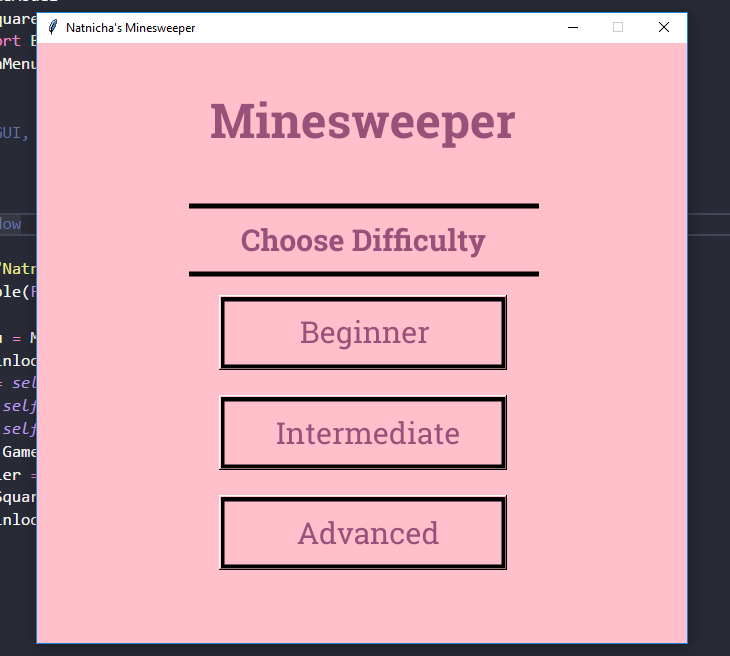
\includegraphics[scale=0.7]{menu}
			\caption{Main menu for mine sweeper: ability to choose difficulty}
		\end{figure}
	
		\begin{figure}[!h]
			\centering
			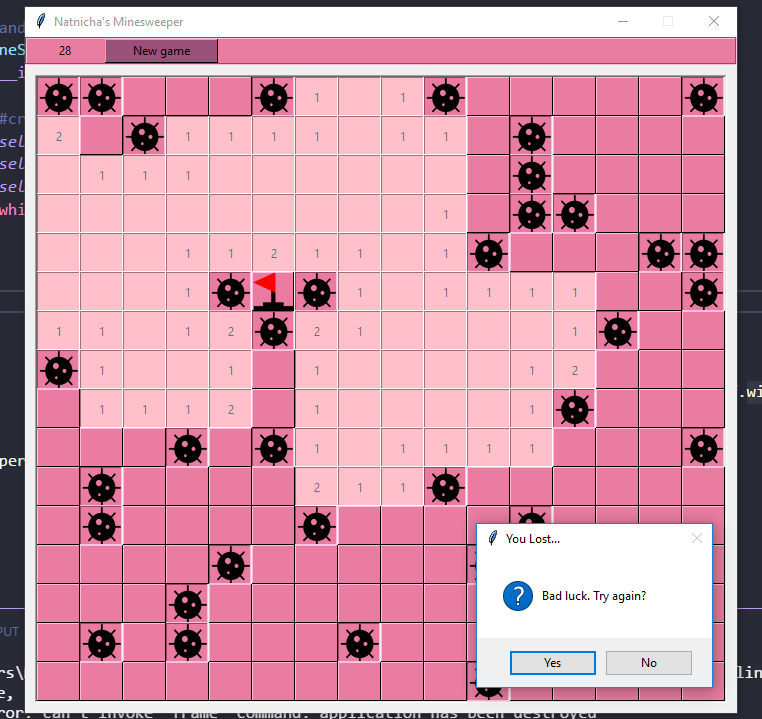
\includegraphics[scale=0.7]{game}
			\caption{Intermediate mode for mine sweeper game: 16 x 16 with 40 mines}
		\end{figure}
	\par The current  version of minesweeper successfully meets the requirements of the traditional minesweeper game. 
 
		\newpage
	\subsection{Cross platform}
	\par The programming language chosen - Python allows the program to be executable on Windows and Linux. The Graphic User Interface (GUI) modules are available to both platforms. Therefore, when creating a program that requires a GUI, Python was considered first when accounting for cross-platform applications. 
	
	\section{Software Development Practices}
	\subsection{Version Control History / Log}
	\begin{tabular}{ | p{3cm} | p{2cm} | p{11cm} | }
		\hline
		Date & User & Activity \\
		\hline
		Sep 22, 2017 & Natnicha & Modified button bindings to deal with left and right handler properly. \\
		Sep 22, 2017 & Natnicha & Ajusted model to refer to boolean list for toggled and flagged for left and right click. \\
		Sep 21, 2017 & Natnicha & Finalised MainMenu class. Destroys Frame after selecting difficulty. \\
		Sep 20, 2017 & Natnicha & MainMenu class: created set difficulty function to be passed to the model. \\
		Sep 19, 2017 & Natnicha & Finalised Button Controller class to be a Facade for model. \\
		Sep 15, 2017 & Natnicha & Imported images for Main Menu. \\
		Sep 5, 2017 & Natnicha & Made all views extend tkinter.Frame. \\
		Sep 5, 2017 & Natnicha & Added MainMenu class, extends tkinter.Frame. \\ 
		Sep 4, 2017 & Natnicha & Resolved Merging conflict. \\ 
		\hline
	\end{tabular}

	\begin{tabular}{ | p{3cm} | p{2cm} | p{11cm} | }
		\hline
		Sep 4, 2017 & Natnicha & Added diagrams to Report \\ 
		Sep 3, 2017 & Natnicha & Separated create board function in three separate functions for low coupling, removed nested functions. \\ 
		Sep 2, 2017 & Natnicha & Added UML section to report. Put MV files into classes. \\ 
		Sep 1, 2017 & Natnicha & Added timer and reset button functions to Program. \\ 
		Sep 1, 2017 & Natnicha & Added test section to Report. \\ 
		Aug 31, 2017 & Natnicha & Modified test file and fixed formatting in report. Restructured program into MVC architecture. \\ 
		Aug 31, 2017 & Natnicha & Merging conflict resolved. \\
		Aug 31, 2017 & Natnicha & Merging files \\ 
		Aug 30, 2017 & Natnicha & Modified Software Architecture section in Report. \\ 
		Aug 30, 2017 & Natnicha & Completed use case progression and added software architecture section to Report. \\ 
		Aug 30, 2017 & Natnicha & Added more use cases. \\ 
		Aug 30, 2017 & Natnicha & Modified activation button function to handle functionality depending on the backing grid \\ 
		Aug 29, 2017 & Natnicha & Added game end function to handle the program when the game is over. \\ 
		Aug 29, 2017 &Natnicha & Fixed cascading reveal to display empty cells and cells adjacent to. \\ 
		Aug 29, 2017 & Natnicha & Added colour scheme to GUI minesweeper.py \\
		Aug 26, 2017 & Natnicha & Added images to buttons for GUI. \\ 
		\hline
	\end{tabular}
	
	\par \vspace{1cm}\small Note: Repository is private. \textbar{} This log was created by using the command \begin{lstlisting} 
	git log --pretty=format:`%h;%an;%s' > ./log.csv\end{lstlisting}
	
	The development of this program required the use of version control software to save versions of the project and also to monitor/measure productivity. GitHub was created as an online hosting solution for git repositories. Git records a log of past commits pushed to the repository which allows for backtracking of file versions.
	\section{Design Principles}
	\subsection{Least privilege and fail-safe defaults}
	\par
	
	\subsection{Separation of concerns and information hiding}
	\par
	
	\subsection{Coupling, cohesion and encapsulation}
	\par
	
	\section{Design Process}
	\par
	The minesweeper project required a lot of flexibility as the developer had to experiment the GUI class Tkinter and also learn the Model-view controller architecture. The design process used an agile software development method, which is based on the idea that successful development would happen quickly as testing was done regularly. In contrast, the waterfall development process is a more traditional process however, due to the time constraint and also due the low complexity of the system, there was no need to complete processes periodically. The furthest the software process would've progressed to was programming and unit testing. Using agile development, bugs, complications and feature changes are handled better to meet the requirements.
	
	\section{System Models}

	\begin{figure}[!h]
		\centering
		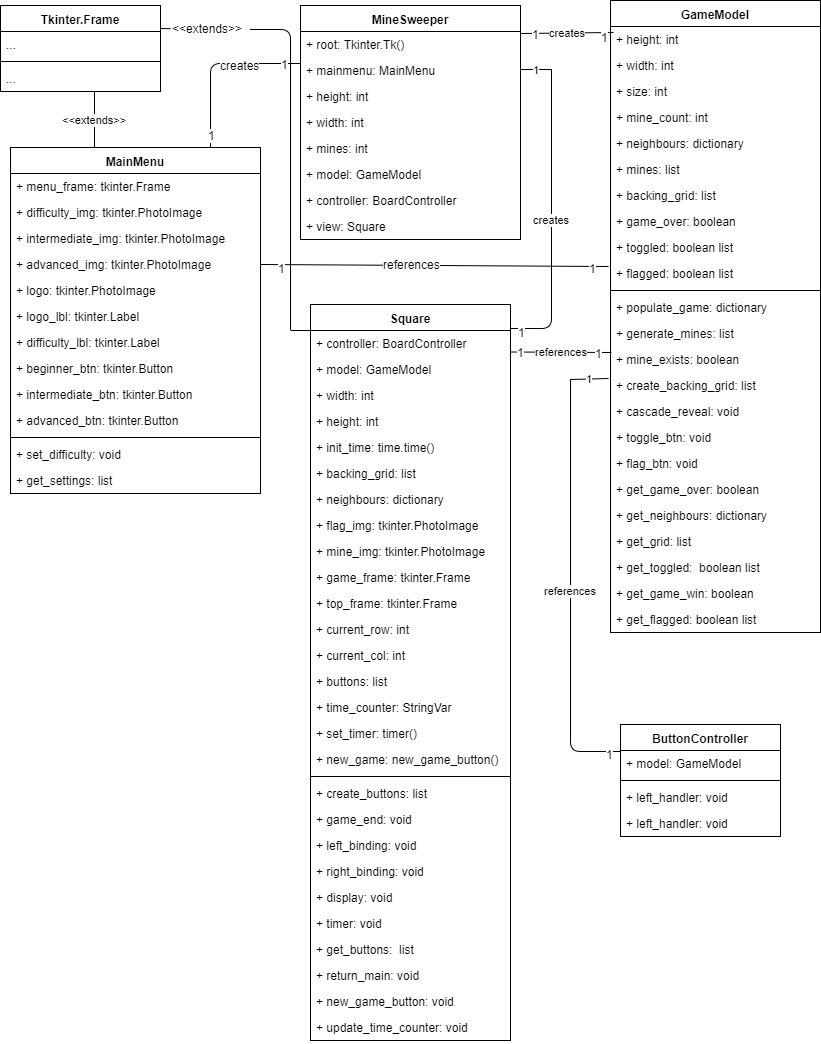
\includegraphics[scale=0.5]{classdiagram}
		\caption{Class diagram for Python implementation of Minesweeper using MVC architecture}
	\end{figure}
	\pagebreak
	
	\begin{figure}[!h]
		\lstinputlisting[language=Python, firstline=1, lastline=26]{minesweeper.txt}
		\caption{Main class Minesweeper}
	\end{figure}
	
	\par The program creates an object of each class in order of what needed to be called from first. Since the views extend tkinter's Frame component, the root frame (main frame) needed to be created first to store the views inside. The main menu object was then created as that was the first view for the game and the main loop is executed. The user selects a difficulty and the initial view's frame is destroyed and the quits. This gives the opportunity to create the model object, which the data is stored, the controller which is a facade for the model and the view which will generate the new frame for game play. The root then executes the main loop once again. 
	
	\section{Design Paradigm}

	\section{Software Architecture}
	
	\section{Design Patterns}
	\par The model-view controller heavily uses the Observer pattern especially in the Model and View. When the data in the model class is modified, the view class needs to be notified and updated as it is run. 
	The Board Controller class uses a Facade design pattern. The facade design pattern simplifies the interface to the model, which can be said to be a complex system. It abstracts the implementation and acts like a proxy, shielding the user from the details stored in the model. Instead leaving the controller to manage between the view and controller. This decouples the program that uses the system from the details of the subsystem, increasing efficiency and understanding for modification later on. 

	\section{User Interface}
	The user interface uses an event driven based design. There is an event and a listener, the listener is notified when an event occurs by button click. The event which is bind to the button using an event-handler. The program binds each click to a button. As the player interacts with the game, the game is played with the event of a button press. The event handler function reacts depending on the hidden backing board and the minesweeper board is modified in one of the four different ways. The first way the board can be modified is by clicking a button with a number, which only reveals its own underlying square. The second way is for the square to be empty which checks adjacent squares if they are also empty, this check is done in the cascade reveal function. Thirdly, the underlying cell could be a mine ultimately disabling the state of the board and ending the game. Lastly, the user can flag the square and not activate the button at all but uses the right mouse click event to bind the flag as an overlaying image. 
	
	\section{Model-View Controller}
	\par Model view controller (MVC) is an architecture that allows different parts of a system to be loosely coupled (or separated). MVC keeps the code well-organised into three distinctly different sections of code. Views display data from the model and take user actions. Models represent the data and domain logic in the system. And controllers liaise between the View and the Model, often controlling flow. MVC have separated functions will solve the most common software problems of today: readability, modularity, and coupling. This helps programmers reuse and change code as they are able to work in smaller subset that may be more or less isolated from the larger piece of code or functionality. This structure also helps when testing the program, especially unit testing when sections of code need to be tested. As similar code is sectioned into groups, there is better coverage of test cases. 
	
	\section{Good Software Design}
	\par A good software design should correctly implement all the requirements and functionalities defined in Software Requirement Specification document. With no formal methods of design from the start, the software can very quickly become very difficult to manage. We also want to design the software in a way that will ensure the code is reusable. 
	Since each class is a blueprint of the object it creates, the software will have high cohesion, it should only have methods relating to the intention of the class. It is intentionally done this way to make each class purposeful and independent of another. Another way to refer to this is coupling. 
	The goal of good software design is to lower coupling so that when a part of software needs to be changed, it does not effect the other. 
	Although the main menu and the game frame may extend the same root Frame, the program calls the individual menu and game frame to destroy and quit while maintaining the root frame to be passed on and used in the next view. Another good software design concept is modularity. All the functions in the view have the sole purpose of configuring the buttons depending on the state of the model, the model does not do any configuration and independently handles and mutates the data. This purpose helps separate the classes that are not responsible for configuring but for mutating and vice versa.After the deployment of the software, it should be able to be maintained and easily amenable to change which leads onto the next topic, different designs. 
	\newpage
	\section{Different Designs}
	\par For software developers to create a variety of different designs for their program, comments illustrate how other developers may extend or enhance the already completed program by explaining the purpose of each function. Comments create the opportunity for developers to reuse code and it is imperative to fully understand a block of code with a single, simple and concise comment. It is the only way to capture the intention of the code at the time of writing, when going back to the program later on, it is more effective to continue and progress if there is are basic explanations documented on the same page. Figure 3 below shows the functions in the GameModel class and the associated comments.
	
	\begin{figure}[h]
		\lstinputlisting[language=Python, firstline=28, lastline=59]{minesweeper.txt}
		\caption{Some functions in the GameModel class}
	\end{figure}
	
	
	

\end{document}